\documentclass{article}

\usepackage[spanish]{babel}
\usepackage{mathdots}
\usepackage{listings}
\usepackage{color}
\usepackage[numbers,sort&compress]{natbib}
\usepackage{graphicx}
\usepackage{subfigure}
\usepackage{url}
\usepackage{amsmath}
\usepackage{hyperref}
\usepackage[top=15mm, bottom=40mm, left=15mm, right=15mm]{geometry}
\setlength{\parskip}{2mm}
\setlength{\parindent}{0pt}

\setlength{\parskip}{2mm}
\setlength{\parindent}{0pt}
\definecolor{blue}{rgb}{0,0.6,0}
\definecolor{gray}{rgb}{0.3,0.3,0.3}
\definecolor{orange}{rgb}{0.8,0.4,0}
\definecolor{mostaza}{rgb}{0.9,0.8,0.1}

\lstset{ %
  language=R,                     % the language of the code
  basicstyle=\footnotesize,       % the size of the fonts that are used for the code
  numbers=left,                   % where to put the line-numbers
  numberstyle=\tiny\color{gray},  % the style that is used for the line-numbers
  stepnumber=1,                   % the step between two line-numbers. If it's 1, each line
                                  % will be numbered
  numbersep=5pt,                  % how far the line-numbers are from the code
  backgroundcolor=\color{white},  % choose the background color. You must add \usepackage{color}
  showspaces=false,               % show spaces adding particular underscores
  showstringspaces=false,         % underline spaces within strings
  showtabs=false,                 % show tabs within strings adding particular underscores
  frame=single,                   % adds a frame around the code
  rulecolor=\color{black},        % if not set, the frame-color may be changed on line-breaks within not-black text (e.g. commens (green here))
  tabsize=2,                      % sets default tabsize to 2 spaces
  captionpos=b,                   % sets the caption-position to bottom
  breaklines=true,                % sets automatic line breaking
  breakatwhitespace=false,        % sets if automatic breaks should only happen at whitespace
  title=\lstname,                 % show the filename of files included with \lstinputlisting;
                                  % also try caption instead of title
  keywordstyle=\color{orange},      % keyword style
  commentstyle=\color{blue},   % comment style
  stringstyle=\color{mostaza},      % string literal style
  escapeinside={\%*}{*)},         % if you want to add a comment within your code
  morekeywords={*,...}            % if you want to add more keywords to the set
} 

\author{1445183}
\title{Práctica 7: Búsqueda local}
\date{\today}

\begin{document}

\maketitle

\section{Objetivo}
Maximizar la función bidimensional de \textit{g(x,y)} encontrando el valor máximo de \textit{g} por medio del método de ``búsqueda local''.

\section{Descripción}
 Para encontrar el valor máximo de la función \textit{g(x,y)}, se toma como base el código escrito en la práctica 7 \cite{elisaweb7}, se pide como restricciones que los valores de los ejes \textit{x} y \textit{y} deben estar entre \textit{-3} y \textit{3}; cuando \textit {x,y} tienen una ``posición actual"  tienen ocho vecinos de los cuales tomarán la posición del vecino que tenga el valor mayor, de esta manera el valor de la función \textit{g} será el mayor conforme avance en pasos hasta el punto que llegue a tener el valor máximo.

\begin{lstlisting}[language=R]
g <- function(x, y) {
  return(((x + 0.5)^4 - 30 * x^2 - 20 * x + (y + 0.5)^4 - 30 * y^2 - 20 * y)/100)
}

low <- -3
high <- 3
step <- 0.10
puntos <- 15
tmax <- 10^pot
\end{lstlisting}

Para identificar a los vecinos de \textit{g(x,y)} se le añaden al código variables para ubicar la posición y de esta manera se identifique el vecino con mayor valor:

\begin{lstlisting}[language=R]
posiciones <- data.frame(x = double(), y = double(), bestgxy = double())
for (n in 1:puntos) {
  currx <- runif(1, low, high)
  curry <- runif(1, low, high)
  posiciones <- rbind(posiciones, data.frame(x = currx, y = curry, bestgxy = g(currx, curry)))
}
\end{lstlisting}

\newpage

\begin{lstlisting}[language=R]
for (pot in 1:tmax) {
  resulx <- double()
  resuly <- double()
  
  for (n in 1:puntos) {
    delta <- runif(1, 0, step)
    deltax <- c(-delta, 0, delta)
    delta <- runif(1, 0, step)
    deltay <- c(-delta, 0, delta)
    
    #codigo de la practica 4
    vecinosx <- numeric()
    vecinosy <- numeric()
    for (dx in deltax) {
      for (dy in deltay) {
        if (dx != 0 | dy != 0) { # descartar la posicion misma
          vecinosx <- c(vecinosx, dx)
          vecinosy <- c(vecinosy, dy)
        }
      }
    }
    
    tablax <- rbind(resulx, vecinosx + posiciones$x[n])
    tablay <- rbind(resuly, vecinosy + posiciones$y[n])
  }
  
  vecinos <- g(resulx, resuly)
  maxvalue <- max.col(vecinos)
  
  for (i in 1:puntos) {
    posiciones$x[i] <- resulx[i,maxvalue[i]]
    posiciones$y[i] <- resuly[i,maxvalue[i]]
  }
\end{lstlisting}

Para visualizar mejor la búsqueda se realizan 15 réplicas \texttt{puntos}, es decir, 15 diferentes valores de \textit{x,y} desplazándose hasta llegar a la posición máxima.
\newpage


\section{Resultados}

Se puede observar en la figura \ref{figura 1} cómo los puntos (valor de \textit{g}) tienden a dirigirse hacia la posición máxima al aumentar la cantidad de pasos \cite{gif}.
\begin{figure}[htbp]
\centering
\subfigure[]{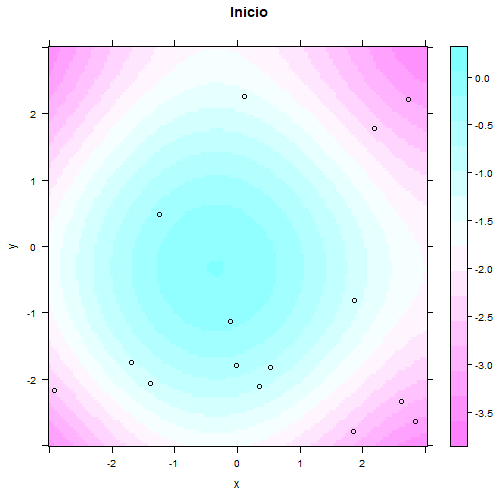
\includegraphics[width=60mm]{./p70.png}}
\subfigure[]{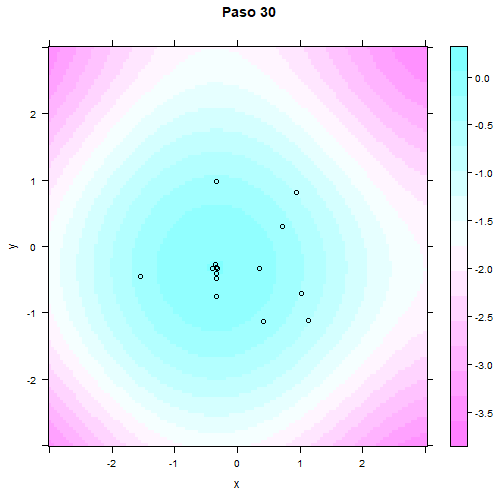
\includegraphics[width=60mm]{./p71.png}}
\subfigure[]{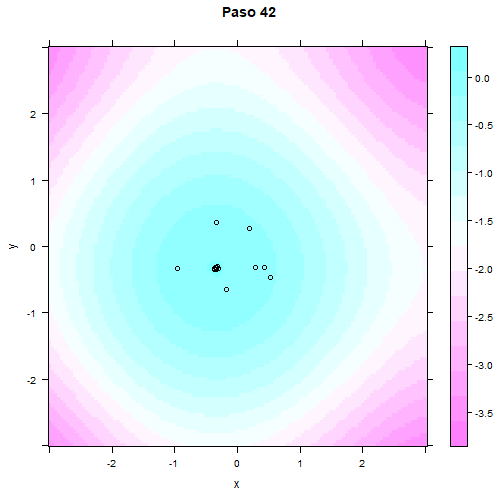
\includegraphics[width=60mm]{./p72.png}}
\subfigure[]{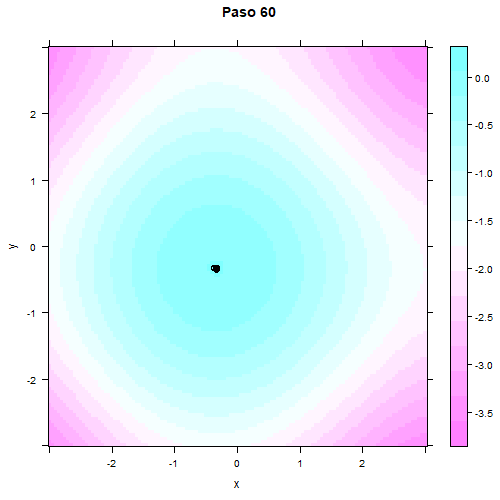
\includegraphics[width=60mm]{./p73.png}}
\caption{Réplicas simultáneas de la búsqueda} \label{figura 1}
\end{figure}





\newpage

\section{Conclusiones}

Una función puede ser optimizada por medio del método de búsqueda local, la cual puede ser un poco parecida al método Monte-Carlo, ya que se observó que a mayor cantidad de pasos la precisión aumenta llegando a un solo valor, aunque en este caso es el valor máximo, es decir, no se puede obtener uno mayor a ese.
El valor máximo se encontró dentro de los primeros 60 pasos auqnue se esperaba obtener una cantidad de pasos mucho mayor. Si hay algún error probablemente sea en los vectores designados para encontrar a los vecinos.


\bibliographystyle{plainnat}
\bibliography{bibliosimu}

\end{document}